%!TEX TS-program = pdflatex
%!TEX root = main.tex
%!TEX encoding = UTF-8 Unicode

\section{Implementation}
\todo[inline]{
  Right now the implementation is subject to change.
  I will complete this section when the source code is stable enough.
}
The code described in this section can be found at
\href{https://github.com/Nyriu/RayTracer}{Nyriu/RayTracer}.

Some images just for showcasing.

\begin{figure}[!htb]
  \centering
  
\includegraphics[width=\linewidth]{img_00.png}
  %\caption{TODO}
  %\label{fig:union}
\end{figure}

\begin{figure}[!htb]
  \centering
  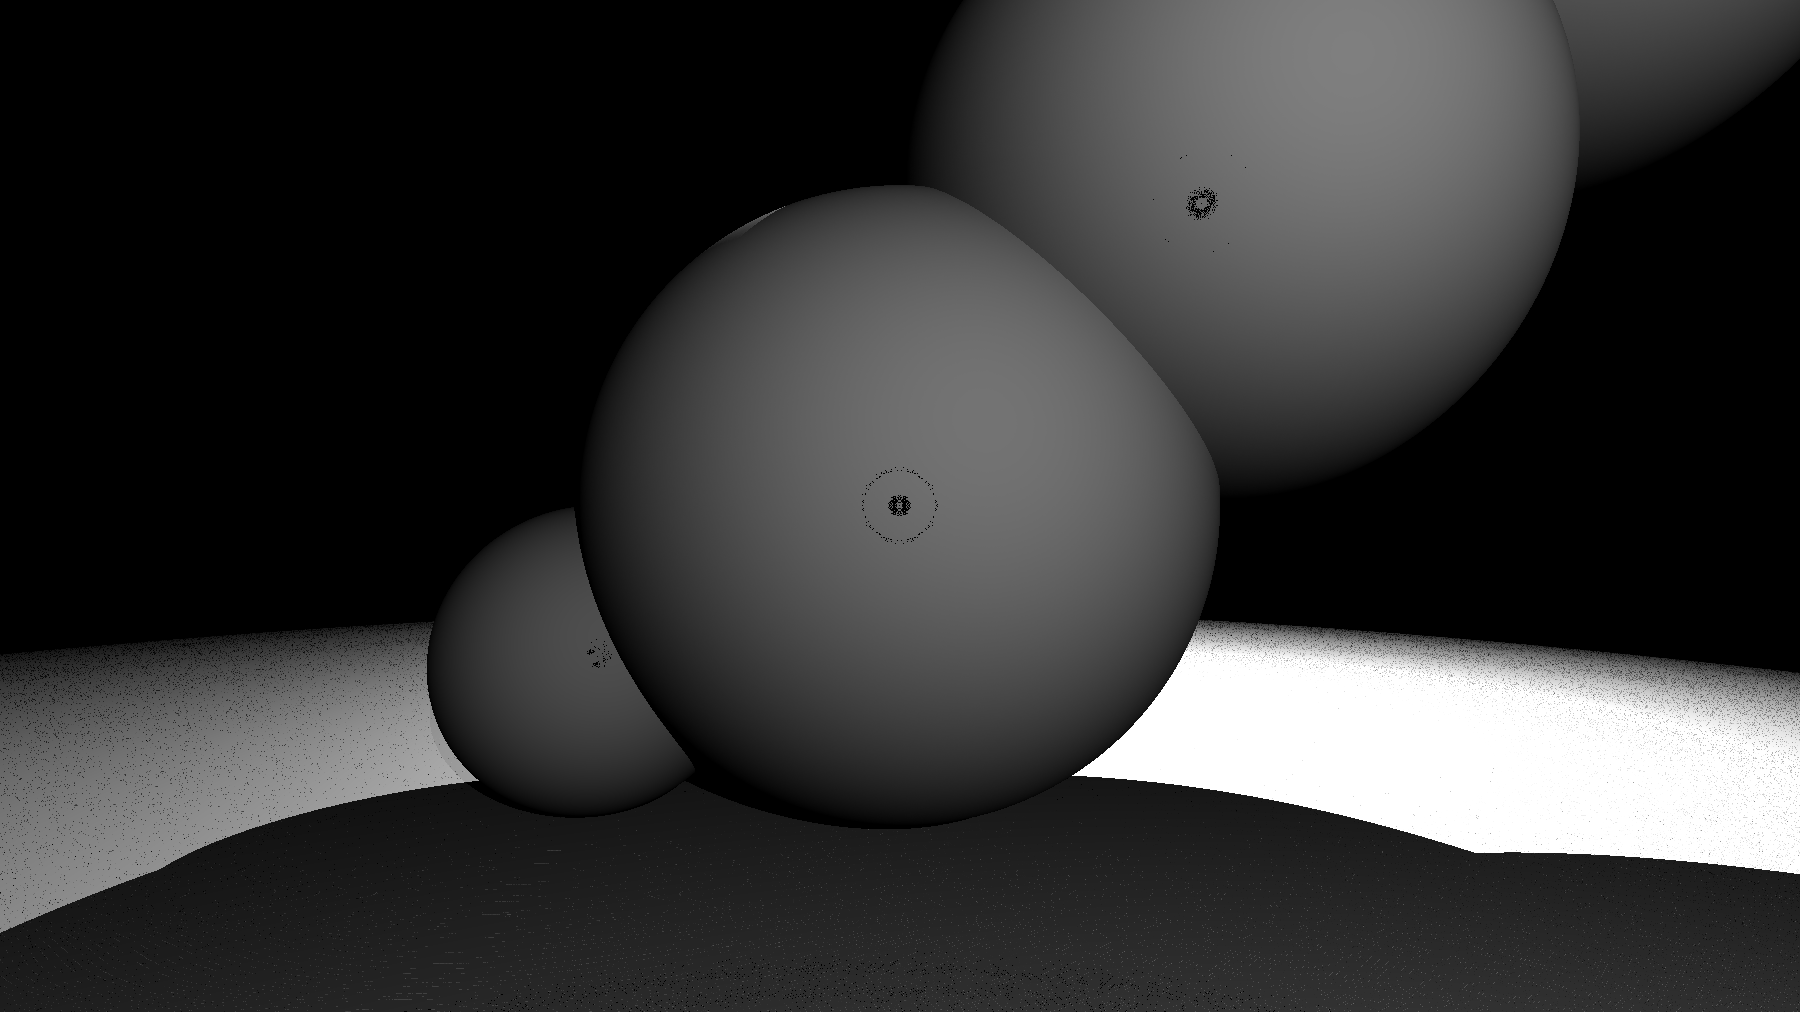
\includegraphics[width=\linewidth]{img_01.png}
  %\caption{TODO}
  %\label{fig:union}
\end{figure}

\begin{figure}[!htb]
  \centering
  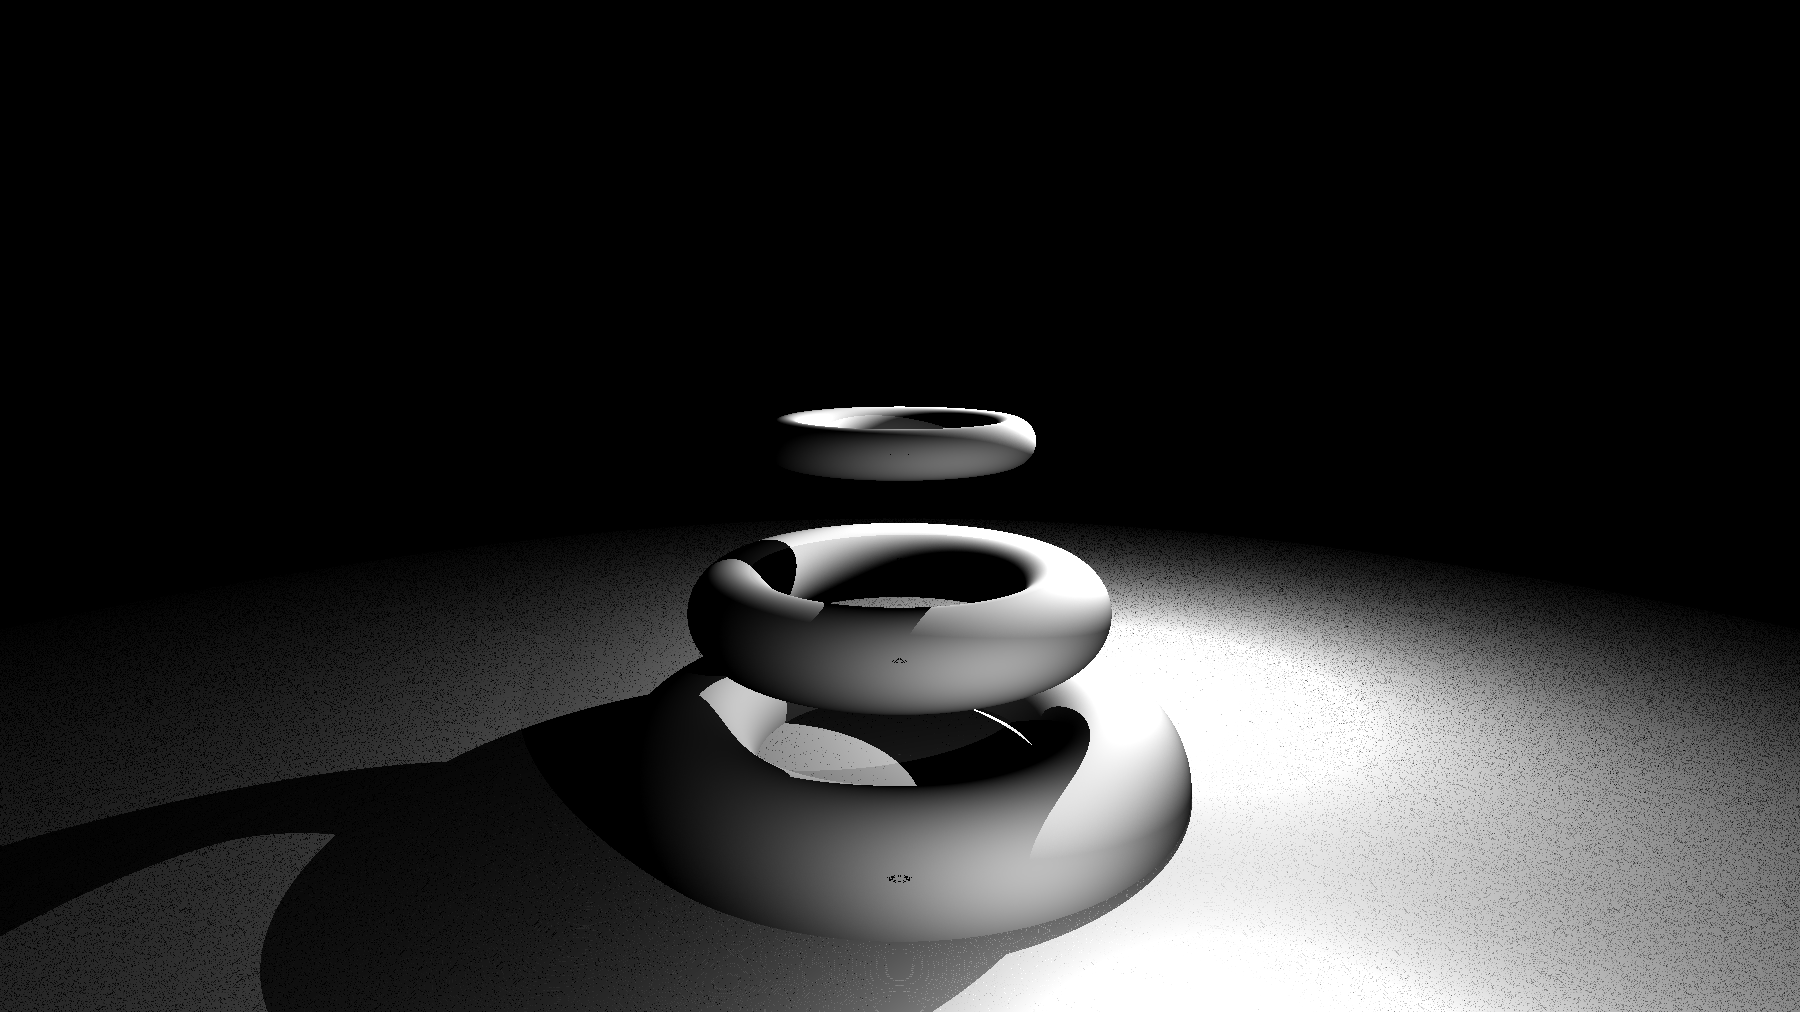
\includegraphics[width=\linewidth]{img_02.png}
  %\caption{TODO}
  %\label{fig:union}
\end{figure}

\begin{figure}[!htb]
  \centering
  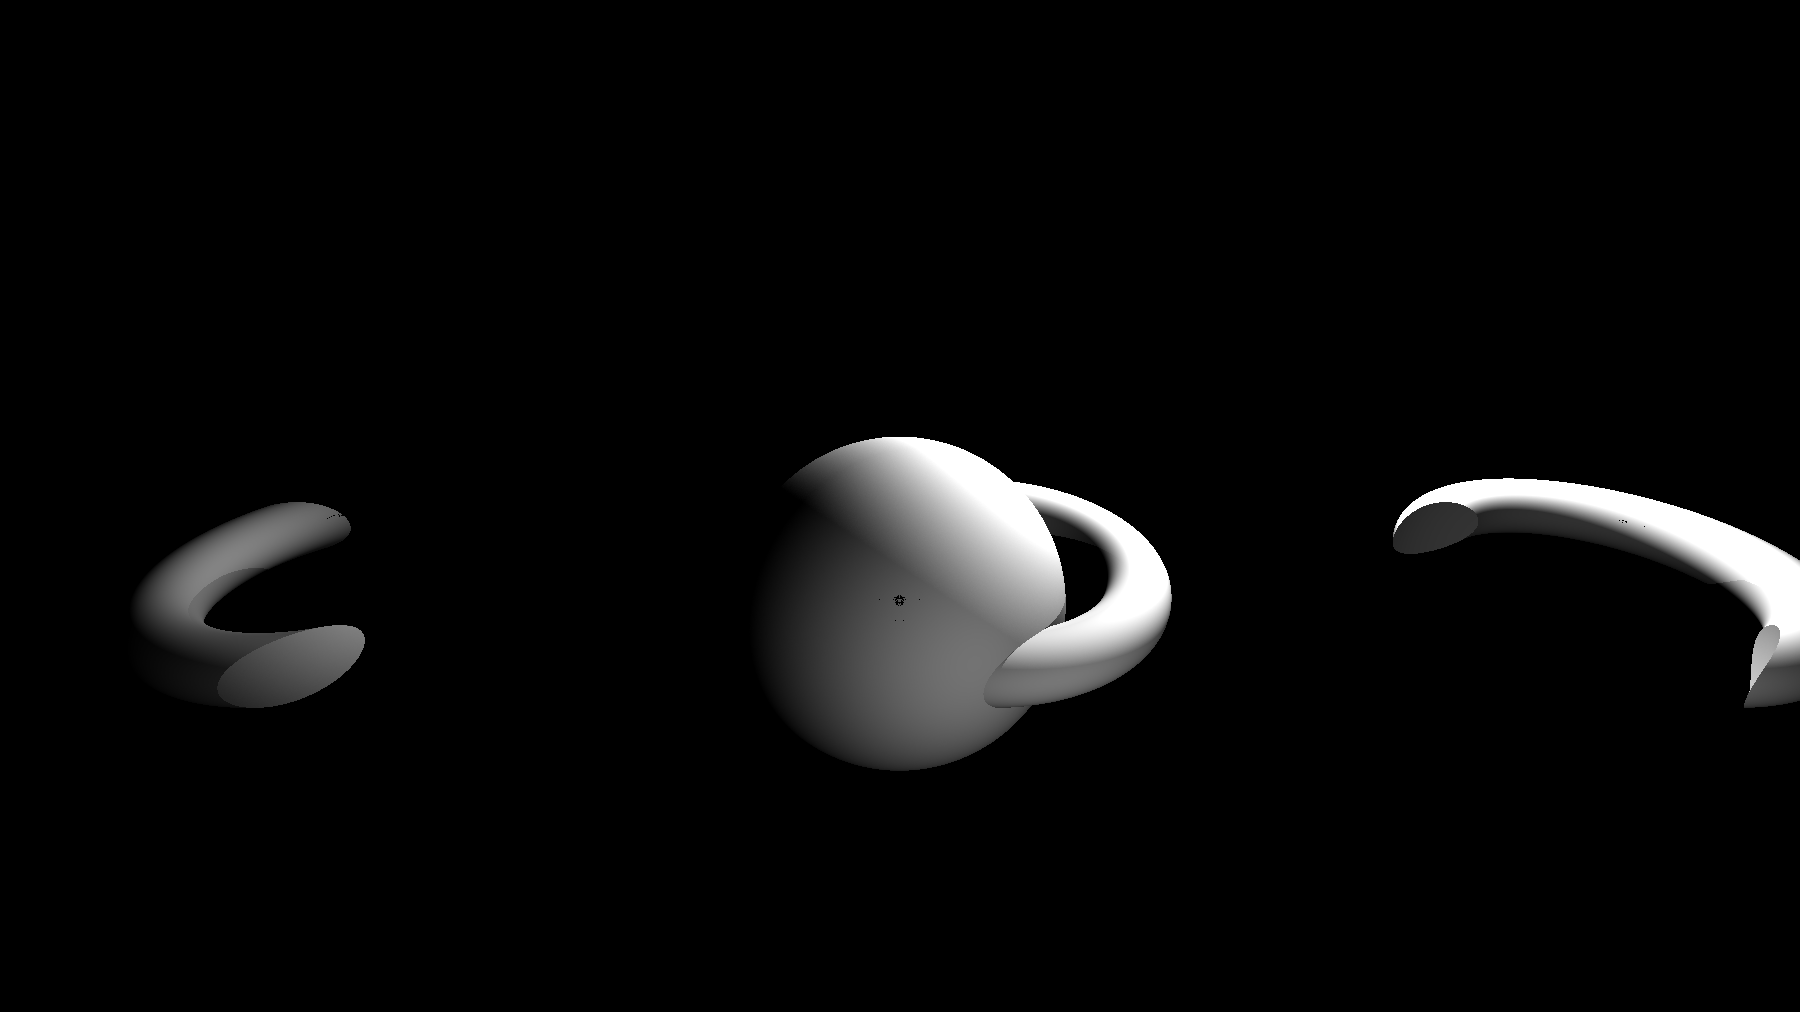
\includegraphics[width=\linewidth]{img_03.png}
  %\caption{TODO}
  %\label{fig:union}
\end{figure}


